% ------------------------------------------------------------------
% Gantt chart of the thesis schedule (TikZ, hand-rolled; no pgfgantt
% dependency). One row per WBS task; x axis in months of 2026.
% DRAFT: bar positions follow the placeholder dates in the WBS table —
% shift them to the official semester calendar before submission.
% ------------------------------------------------------------------
\resizebox{0.92\textwidth}{!}{%
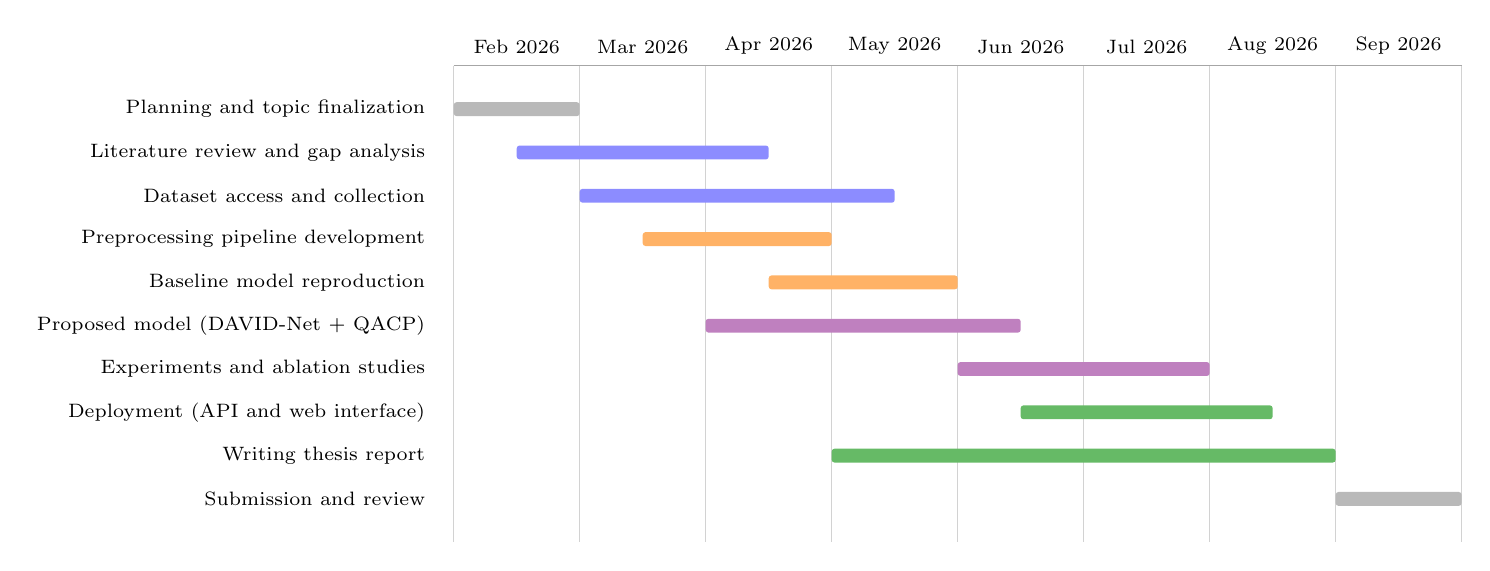
\begin{tikzpicture}[
  font=\scriptsize,
  bar/.style={draw=none, rounded corners=1pt, minimum height=0.32cm},
  x=1.6cm, y=0.55cm
]
% ---- month grid: columns Feb..Sep 2026 (x = 0..8) ----
\foreach \m/\lab in {0/Feb, 1/Mar, 2/Apr, 3/May, 4/Jun, 5/Jul, 6/Aug, 7/Sep}
{
  \draw[gray!35] (\m,0) -- (\m,-11);
  \node[anchor=south] at (\m+0.5, 0.05) {\lab~2026};
}
\draw[gray!35] (8,0) -- (8,-11);

% ---- task rows (y = -1 .. -10) ----
\node[anchor=east] at (-0.15,-1)  {Planning and topic finalization};
\fill[gray!55,  rounded corners=1pt] (0.0,-1.16)  rectangle (1.0,-0.84);

\node[anchor=east] at (-0.15,-2)  {Literature review and gap analysis};
\fill[blue!45,  rounded corners=1pt] (0.5,-2.16)  rectangle (2.5,-1.84);

\node[anchor=east] at (-0.15,-3)  {Dataset access and collection};
\fill[blue!45,  rounded corners=1pt] (1.0,-3.16)  rectangle (3.5,-2.84);

\node[anchor=east] at (-0.15,-4)  {Preprocessing pipeline development};
\fill[orange!60, rounded corners=1pt] (1.5,-4.16) rectangle (3.0,-3.84);

\node[anchor=east] at (-0.15,-5)  {Baseline model reproduction};
\fill[orange!60, rounded corners=1pt] (2.5,-5.16) rectangle (4.0,-4.84);

\node[anchor=east] at (-0.15,-6)  {Proposed model (DAVID-Net + QACP)};
\fill[violet!50, rounded corners=1pt] (2.0,-6.16) rectangle (4.5,-5.84);

\node[anchor=east] at (-0.15,-7)  {Experiments and ablation studies};
\fill[violet!50, rounded corners=1pt] (4.0,-7.16) rectangle (6.0,-6.84);

\node[anchor=east] at (-0.15,-8)  {Deployment (API and web interface)};
\fill[green!55!black!60, rounded corners=1pt] (4.5,-8.16) rectangle (6.5,-7.84);

\node[anchor=east] at (-0.15,-9)  {Writing thesis report};
\fill[green!55!black!60, rounded corners=1pt] (3.0,-9.16) rectangle (7.0,-8.84);

\node[anchor=east] at (-0.15,-10) {Submission and review};
\fill[gray!55,  rounded corners=1pt] (7.0,-10.16) rectangle (8.0,-9.84);

% ---- axis line ----
\draw[gray!70] (0,0) -- (8,0);
\end{tikzpicture}}%
